\section{考察}

弾性接触において,摩擦係数$\mu$が垂直荷重$W$により理論的にどのように変化するか,式(\ref{eq:摩擦係数})からせん断強度$\tau$が一定として考察する.式(\ref{eq:摩擦係数})の分母である$W$が増加すると,接触面の変形により接触面積も増加する.弾性接触では式(\ref{eq:接触円半径})から接触面積は$W$の2/3乗で増加するため,$W$が増加すると分母の増加速度のほうがやや速くなり,摩擦係数は減少していくと考えられる.一方,塑性接触では接触面積が$W$に比例して増加するため,摩擦係数は変化しないと考えられる.

ここで式(\ref{eq:平均接触圧力}),式(\ref{eq:接触円半径})から$P_m$は$W$の増加に伴って増加するので,図\ref{fig:fig_Pm}から実験結果との対応を考察する.
グラフでは弾性接触の範囲である$\mathrm{P_m/H_v}$ = 0から0.36の範囲で摩擦係数が減少する傾向があり,$\mathrm{P_m/H_v}$ = 0.5を過ぎたあたりからほぼ一定値となっている.これはおおよそ理論通りの挙動であると考えることができる.一方,$\mathrm{P_m/H_v}$ = 1.7あたりでは摩擦係数が増加する傾向がみられた.これは,$\mathrm{P_m/H_v}$ = 1を超える塑性接触により,ボール試験片がプレート試験片に対して削るように運動した結果,掘り起こし項の影響が大きくなったためだと考えられる.

ボール試験片をアルミナに変更した場合の摩擦係数の変化を考察する.アルミナに変更した場合の等価縦弾性係数は約64.7[GPa]となり,これは本実験条件における値57.4[GPa]よりも大きい.したがって,式(\ref{eq:接触円半径})から等価縦弾性係数が大きくなると,接触面積が小さくなるため,弾性接触においては摩擦係数は減少すると考えられる.一方,塑性接触の領域ではプレート試験片の方が軟質であるため,接触面積があまり変わらず,摩擦係数は変化しないと考えられる.

逆にプレート試験片をアルミナに変更した場合の摩擦係数の変化を考察する.アルミ合金をアルミナに変更した場合の等価縦弾性係数はさらに大きくなるため,弾性接触の領域では摩擦係数はさらに減少すると考えられる.一方,塑性接触の領域では軸受鋼球のボール試験片のほうが軟質であるため,アルミ合金を使用した際よりも摩擦係数は減少すると考えられる.

すべり方向に対して接触円前端と降誕ではどのような応力状態となっているか考察する.接触円中心を通りすべり方向に平行な線上のすべり方向応力$\sigma_x$は,以下の式で表される.
\begin{equation}
    \label{eq:すべり方向応力}
    \sigma_x = \frac{3W}{2\pi a^2}\lbrack(\frac{1-2\nu}{3})\lbrace\frac{1-(1-x^2)^{\frac{3}{2}}}{x^2}\rbrace - (1 - x^2)^{\frac{1}{2}} - \pi \mu (\frac{4 + \nu}{8})x \rbrack
\end{equation}
ここで$x$は接触半径$a$に対する接触円中心からの位置$d$の相対比である.この式から$x$に対する$\sigma_x$の変化をボール半径1mm,垂直荷重0.98としてプロットしたものを図\ref{fig:fig_Sigma_X}に示す.グラフから接触円前端では接触部よりも強い圧縮応力が生じており,後端では引張応力が生じていると考えられる.

\begin{figure}[htbp]
    \centering %中央揃え
    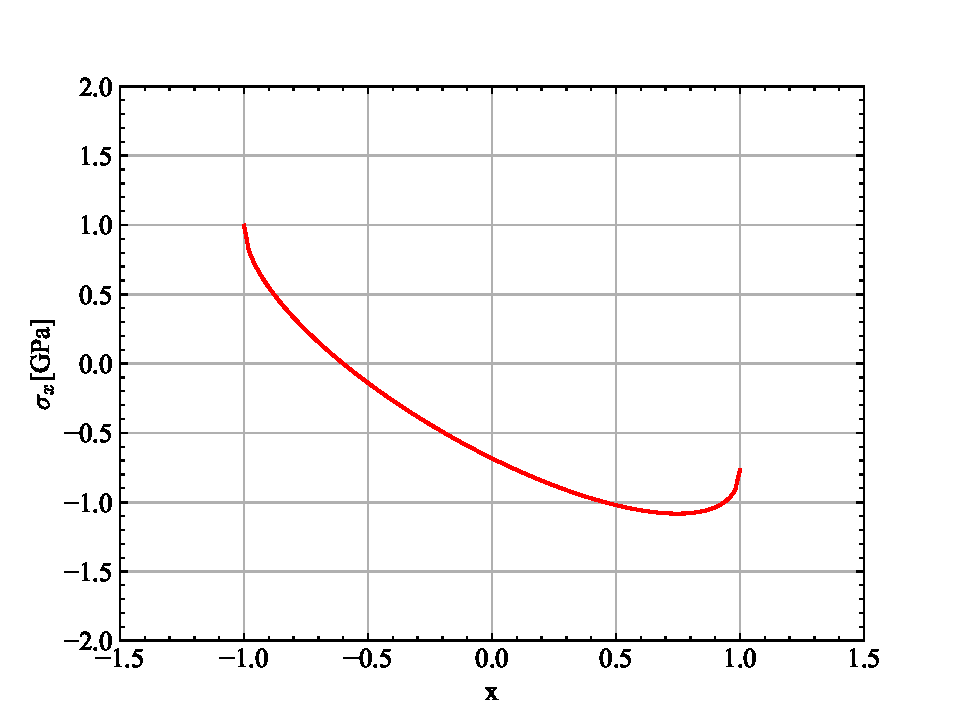
\includegraphics[width=100truemm,clip]{fig/fig_Sigma_X.pdf}
    \caption{Variation of stress in slip direction with respect to x.}
    \label{fig:fig_Sigma_X}
\end{figure}



